\documentclass[12pt, oneside]{article}

\usepackage[letterpaper, scale=0.89, centering]{geometry}
\usepackage{fancyhdr}
\setlength{\parindent}{0em}
\setlength{\parskip}{1em}

\usepackage{tikz}
\usetikzlibrary{automata,positioning,arrows}

\pagestyle{fancy}
\fancyhf{}
\renewcommand{\headrulewidth}{0pt}
\rfoot{\href{https://creativecommons.org/licenses/by-nc-sa/2.0/}{CC BY-NC-SA 2.0} Version \today~(\thepage)}

\usepackage{amssymb,amsmath,pifont,amsfonts,comment,enumerate,enumitem}
\usepackage{currfile,xstring,hyperref,tabularx,graphicx,wasysym}
\usepackage[labelformat=empty]{caption}
\usepackage{xcolor}
\usepackage{multicol,multirow,array,listings,tabularx,lastpage,textcomp,booktabs}

\lstnewenvironment{algorithm}[1][] {   
    \lstset{ mathescape=true,
        frame=tB,
        numbers=left, 
        numberstyle=\tiny,
        basicstyle=\rmfamily\scriptsize, 
        keywordstyle=\color{black}\bfseries,
        keywords={,procedure, div, for, to, input, output, return, datatype, function, in, if, else, foreach, while, begin, end, }
        numbers=left,
        xleftmargin=.04\textwidth,
        #1
    }
}
{}

\newcommand\abs[1]{\lvert~#1~\rvert}
\newcommand{\st}{\mid}

\newcommand{\cmark}{\ding{51}}
\newcommand{\xmark}{\ding{55}}
 
\begin{document}
\begin{flushright}
    \StrBefore{\currfilename}{.}
\end{flushright} \section*{Week4 monday}


Regular sets are not the end of the story
\begin{itemize}
    \item Many nice / simple / important sets are not regular
    \item Limitation of the finite-state automaton model: Can't ``count", Can only remember finitely far into the past,
    Can't backtrack, Must make decisions in ``real-time"
    \item We know actual computers are more powerful than this model...
\end{itemize}

The {\bf next} model of computation. Idea: allow some memory of unbounded size. How? 
\begin{itemize}
    \item To generalize regular expressions: {\bf context-free grammars}\\
    \item To generalize NFA: {\bf Pushdown automata}, which is like an NFA with access to a stack: 
    Number of states is fixed, number of entries in stack is unbounded. At each step
    (1) Transition to new state based on current state, letter read, and top letter of stack, then
    (2) (Possibly) push or pop a letter to (or from) top of stack. Accept a string iff
    there is some sequence of states and some sequence of stack contents 
    which helps the PDA processes the entire input string and ends in an accepting state.
\end{itemize}

\vfill

\vfill

Is there a PDA that recognizes the nonregular language $\{0^n1^n \mid n \geq 0 \}$?

\vfill

\newpage

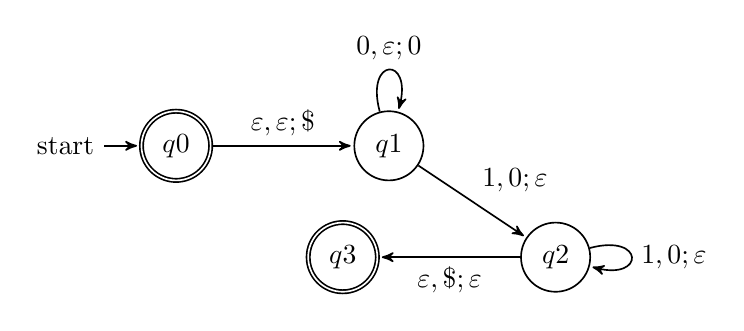
\begin{tikzpicture}[->,>=stealth',shorten >=1pt, auto, node distance=2cm, semithick]
    \tikzstyle{every state}=[text=black, fill=none]
    
    \node[initial,state,accepting] (q0)          {$q0$};
    \node[state]         (q1) [right of=q0, xshift=20pt] {$q1$};
    \node[state]         (q2) [below right of=q1, xshift=20pt] {$q2$};
    \node[state,accepting]         (q3) [left of=q2, xshift=-20pt] {$q3$};
    
    \path (q0) edge [bend left=0] node {$\varepsilon, \varepsilon; \$$} (q1)
        (q1) edge  [loop above] node {$0, \varepsilon; 0$} (q1)
        (q1) edge [bend left=0] node {$1, 0; \varepsilon$} (q2)
        (q2) edge  [loop right] node {$1, 0; \varepsilon$} (q2)
        (q2) edge  [bend left=0] node {$\varepsilon, \$; \varepsilon$} (q3)
    ;
\end{tikzpicture}

The PDA with state diagram above can be informally described as:
\begin{quote}
    Read symbols from the input. As each 0 is read, push it onto the stack. 
    As soon as 1s are seen, pop a 0 off the stack for each 1 read. 
    If the stack becomes empty and we are at the end of the input string, accept the input. 
    If the stack becomes empty and there are 1s left to read, 
    or if 1s are finished while the stack still contains 0s, or if any 0s
    appear in the string following 1s, 
    reject the input.
\end{quote}
    

Trace the computation of this PDA on the input string $01$.

\vfill
    
Trace the computation of this PDA on the input string $011$.

\vfill

\newpage
A PDA recognizing the set $\{ \hspace{1.5 in} \}$ can be informally described as:
\begin{quote}
    Read symbols from the input. As each 0 is read, push it onto the stack. 
    As soon as 1s are seen, pop a 0 off the stack for each 1 read. 
    If the stack becomes empty and there is exactly one 1 left to read, read that 1 and accept the input. 
    If the stack becomes empty and there are either zero or more than one 1s left to read, 
    or if the 1s are finished while the stack still contains 0s, or if any 0s appear in the input following 1s, 
    reject the input.
\end{quote}
Modify the state diagram below to get a PDA that implements this description:

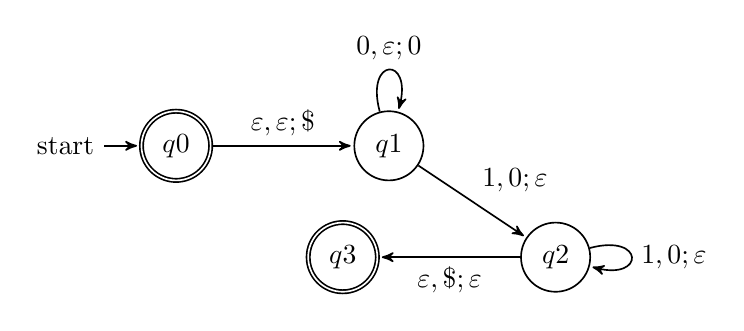
\begin{tikzpicture}[->,>=stealth',shorten >=1pt, auto, node distance=2cm, semithick]
    \tikzstyle{every state}=[text=black, fill=none]
    
    \node[initial,state,accepting] (q0)          {$q0$};
    \node[state]         (q1) [right of=q0, xshift=20pt] {$q1$};
    \node[state]         (q2) [below right of=q1, xshift=20pt] {$q2$};
    \node[state,accepting]         (q3) [left of=q2, xshift=-20pt] {$q3$};
    
    \path (q0) edge [bend left=0] node {$\varepsilon, \varepsilon; \$$} (q1)
        (q1) edge  [loop above] node {$0, \varepsilon; 0$} (q1)
        (q1) edge [bend left=0] node {$1, 0; \varepsilon$} (q2)
        (q2) edge  [loop right] node {$1, 0; \varepsilon$} (q2)
        (q2) edge  [bend left=0] node {$\varepsilon, \$; \varepsilon$} (q3)
    ;
\end{tikzpicture}
    
 \vfill
\section*{Week4 wednesday}



{\bf Definition} A {\bf pushdown automaton} (PDA) is  specified by a  $6$-tuple $(Q, \Sigma, \Gamma, \delta, q_0, F)$
where $Q$ is the finite set of states, $\Sigma$ is the input alphabet,  $\Gamma$ is the stack alphabet,
\[
    \delta: Q \times \Sigma_\varepsilon  \times  \Gamma_\varepsilon \to \mathcal{P}( Q \times \Gamma_\varepsilon)
\]
is the transition function,  $q_0 \in Q$ is the start state, $F \subseteq  Q$ is the set of accept states.


Draw the state diagram and give the formal definition of a PDA with $\Sigma = \Gamma$.

\vfill

Draw the state diagram and give the formal definition of a PDA with $\Sigma \cap \Gamma = \emptyset$.
    
\vfill

\newpage
For the PDA state diagrams below, $\Sigma = \{0,1\}$.


\begin{center}
\begin{tabular}{c c}
Mathematical description of language & State diagram of PDA recognizing language\\
\hline
& $\Gamma = \{ \$, \#\}$ \hspace{2.3in} \\
& \\
& 
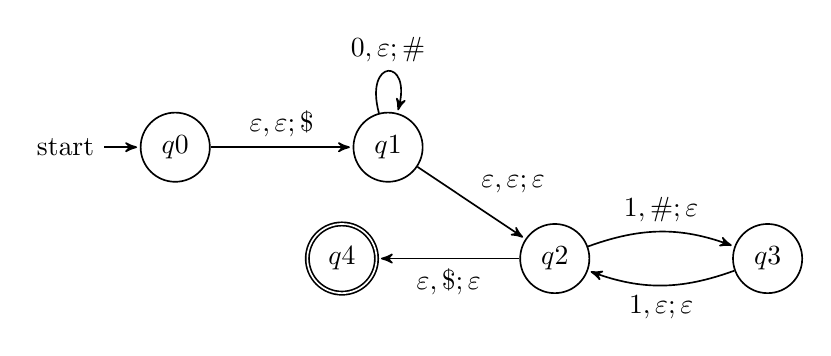
\begin{tikzpicture}[->,>=stealth',shorten >=1pt, auto, node distance=2cm, semithick]
    \tikzstyle{every state}=[text=black, fill=none]
    
    \node[initial,state] (q0)          {$q0$};
    \node[state]         (q1) [right of=q0, xshift=20pt] {$q1$};
    \node[state]         (q2) [below right of=q1, xshift=20pt] {$q2$};
    \node[state]         (q3) [right of=q2, xshift=20pt] {$q3$};
    \node[state,accepting]         (q4) [left of=q2, xshift=-20pt] {$q4$};
    
    \path (q0) edge [bend left=0] node {$\varepsilon, \varepsilon; \$$} (q1)
        (q1) edge  [loop above] node {$0, \varepsilon; \#$} (q1)
        (q1) edge [bend left=0] node {$\varepsilon, \varepsilon; \varepsilon$} (q2)
        (q2) edge  [bend left=20] node [midway, above] {$1, \#; \varepsilon$} (q3)
        (q3) edge  [bend left=20] node [midway, below] {$1, \varepsilon; \varepsilon$} (q2)
        (q2) edge  [bend left=0] node {$\varepsilon, \$; \varepsilon$} (q4)
    ;
\end{tikzpicture}
\\
& \\
& \\
\hline
& $\Gamma = \{ \sun, 1\}$ \hspace{2.3in} \\
& \\
& 
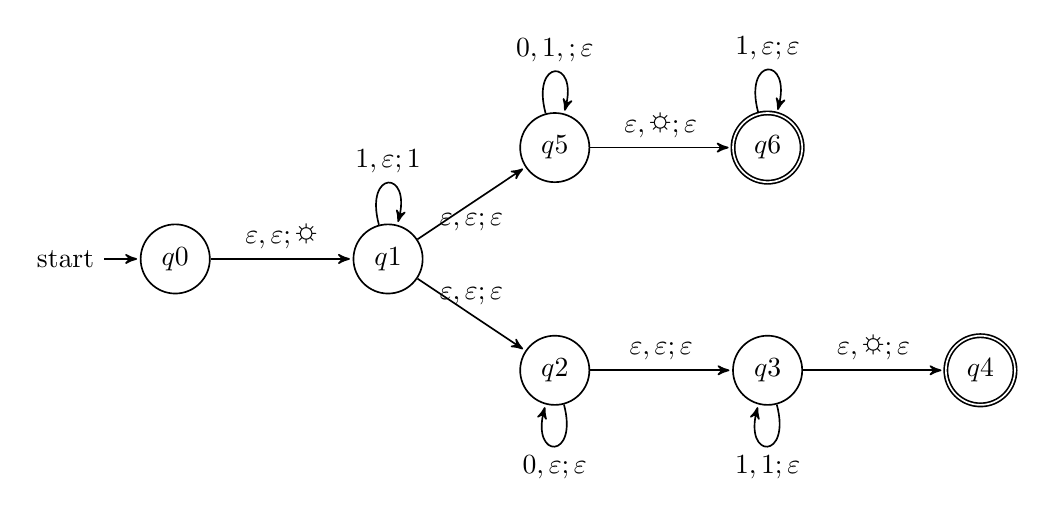
\begin{tikzpicture}[->,>=stealth',shorten >=1pt, auto, node distance=2cm, semithick]
    \tikzstyle{every state}=[text=black, fill=none]
    
    \node[initial,state] (q0)          {$q0$};
    \node[state]         (q1) [right of=q0, xshift=20pt] {$q1$};
    \node[state]         (q2) [below right of=q1, xshift=20pt] {$q2$};
    \node[state]         (q3) [right of=q2, xshift=20pt] {$q3$};
    \node[state,accepting]  (q4) [right of=q3, xshift=20pt] {$q4$};
    \node[state]         (q5) [above right of=q1, xshift=20pt] {$q5$};
    \node[state,accepting]  (q6) [right of=q5, xshift=20pt] {$q6$};
    
    \path (q0) edge [bend left=0] node {$\varepsilon, \varepsilon; \sun$} (q1)
        (q1) edge  [loop above] node {$1, \varepsilon; 1$} (q1)
        (q1) edge [bend left=0] node [below] {$\varepsilon, \varepsilon; \varepsilon$} (q5)
        (q1) edge [bend left=0] node [above]{$\varepsilon, \varepsilon; \varepsilon$} (q2)
        (q5) edge [loop above] node {$0, 1, ; \varepsilon$} (q5)
        (q5) edge [bend left=0] node {$\varepsilon, \sun; \varepsilon$} (q6)
        (q6) edge [loop above] node {$1, \varepsilon; \varepsilon$} (q6)
        (q2) edge [loop below] node {$0, \varepsilon; \varepsilon$} (q2)
        (q2) edge  [bend left=0] node {$\varepsilon, \varepsilon; \varepsilon$} (q3)
        (q3) edge  [loop below] node {$1, 1; \varepsilon$} (q3)
        (q3) edge  [bend left=0] node {$\varepsilon, \sun; \varepsilon$} (q4)
    ;
\end{tikzpicture}
\\
& \\
& \\
\hline
& \\
& \\
& \\
$\{ 0^i 1^j 0^k \mid i,j,k \geq 0 \}$ & \\
& \\
& \\
\end{tabular}
\end{center}

 \vfill
 {\it Note: alternate notation is to replace $;$ with $\to$}

\begin{comment}
{\it Extra practice}: Consider the state diagram of a PDA with input alphabet 
$\Sigma$ and stack alphabet $\Gamma$.

\begin{center}
\begin{tabular}{|c|c|}
\hline
Label & means \\
\hline
$a, b ; c$ when $a \in \Sigma$, $b\in \Gamma$, $c \in \Gamma$ 
& \hspace{3in} \\
& \\
& \\
& \\
& \\
&\\
\hline
$a, \varepsilon ; c$ when $a \in \Sigma$, $c \in \Gamma$ 
& \hspace{3in} \\
& \\
& \\
& \\
& \\
&\\
\hline
$a, b ; \varepsilon$ when $a \in \Sigma$, $b\in \Gamma$
& \hspace{3in} \\
& \\
& \\
& \\
& \\
&\\
\hline
$a, \varepsilon ; \varepsilon$ when $a \in \Sigma$
& \hspace{3in} \\
& \\
& \\
& \\
& \\
&\\
\hline
\end{tabular}
\end{center}


How does the meaning change if $a$ is replaced by $\varepsilon$?
\end{comment}
 \vfill
\section*{Week4 friday}



{\it Big picture}: PDAs were motivated by wanting to add some memory of unbounded size to NFA. How 
do we accomplish a similar enhancement of regular expressions to get a syntactic model that is 
more expressive?

DFA, NFA, PDA: Machines process one input string at a time; the computation of a machine on its input string 
reads the input from left to right.

Regular expressions: Syntactic descriptions of all strings that match a particular pattern; the language 
described by a regular expression is built up recursively according to the expression's syntax

{\bf Context-free grammars}: Rules to produce one string at a time, adding characters from the middle, beginning, 
or end of the final string as the derivation proceeds.\\



Definitions below are on pages 101-102.

\vspace{-20pt}

\begin{center}
    \begin{tabular}{|p{2.4in}cp{3.6in}|}
    \hline 
    {\bf Term} & {\bf Typical symbol} & {\bf Meaning} \\
     & or {\bf Notation} & \\
    \hline
    \hline
    {\bf Context-free grammar} (CFG) & $G$ & $G = (V, \Sigma, R, S)$ \\
    The set of {\bf variables}& $V$ & Finite  set of symbols that represent phases in production pattern\\
    The set of {\bf terminals} & $\Sigma$ & Alphabet of symbols of strings generated  by CFG \\
    & & $V \cap \Sigma = \emptyset$ \\
    The set of {\bf rules}& $R$ & Each rule is  $A \to u$ with $A \in V$ and $u  \in (V  \cup \Sigma)^*$\\
    The {\bf start} variable&  $S$  & Usually  on left-hand-side of first/ topmost rule \\
    & &\\
    {\bf Derivation} & $S \Rightarrow \cdots \Rightarrow w$& 
    Sequence  of substitutions in a  CFG (also written $S \Rightarrow^* w$). At each step, we can apply one rule 
    to one occurrence of a variable in the current string by substituting that occurrence of the variable with the 
    right-hand-side of the rule. The derivation must end when the current string has only terminals (no variables)
    because then there are no instances of variables to apply a rule to.\\
    Language {\bf generated} by the context-free grammar $G$ & $L(G)$ &The set of strings for which there is a derivation in $G$. 
    Symbolically: $\{  w \in \Sigma^* \mid S \Rightarrow^* w \}$ i.e. $$\{  w \in \Sigma^* \mid \text{there is  derivation in $G$ that ends
    in $w$} \}$$\\
    {\bf Context-free language} & & A language that is the language generated by some context-free grammar\\
    \hline
    \end{tabular}
\end{center}

\vfill

\newpage
  
{\bf Examples of context-free grammars, derivations in those grammars, and the languages generated by those grammars}
  
$G_1 =  (\{S\}, \{0\}, R, S)$ with rules
  \begin{align*}
    &S \to 0S\\
    &S \to 0\\
  \end{align*}
  In  $L(G_1)$ \ldots 
  
\vfill

  Not in $L(G_1)$ \ldots 


  \vfill

\newpage
  $G_2 =  (\{S\}, \{0,1\}, R, S)$
  \[
  S \to 0S \mid 1S \mid \varepsilon
  \]
  In  $L(G_2)$ \ldots 
  
  \vspace{110pt}
  
  Not in $L(G_2)$ \ldots 

  \vspace{110pt}

  $(\{S, T\}, \{0, 1\}, R, S)$ with  rules
  \begin{align*}
  &S \to T1T1T1T \\
  &T \to  0T \mid 1T \mid \varepsilon
  \end{align*}

  In  $L(G_3)$ \ldots 
  
  \vspace{110pt}
  
  Not in $L(G_3)$ \ldots 

  \vspace{110pt}

\newpage
  $G_4 =  (\{A, B\}, \{0, 1\}, R, A)$ with rules
  \[
    A \to 0A0 \mid  0A1 \mid 1A0  \mid 1A1 \mid  1
  \]
  In  $L(G_4)$ \ldots 
  
  \vspace{110pt}
  
  Not in $L(G_4)$ \ldots 

  \vspace{110pt}


  \begin{comment}
    I moved the following to the review quiz.

    {\it Extra practice}: Is there a CFG $G$ with $L(G) = \emptyset$?


  Three different CFGs that each generate the  language $\{abba\}$
  
  \begin{align*}
  & ( \{ S, T, V, W\}, \{a,b\}, \{ S \to aT, T \to bV, V \to bW, W \to a\}, S)\\
  & \\ 
  & \\ 
  & \\ 
  & ( \{ Q \}, \{a,b\}, \{Q \to abba\}, Q) \\
  & \\ 
  & \\ 
  & \\
  & ( \{ X,Y \}, \{a,b\}, \{X \to aYa, Y \to bb\}, X) 
  & \\ 
  & \\ 
  \end{align*} 
\end{comment}
  \newpage
  Design a CFG to generate the  language $\{a^n b^n \mid  n  \geq  0\}$
  
  \vspace{100pt}
  
  {\it Sample derivation:} 
  
  \vspace{100pt}
  
  
  \vfill 


\newpage
 \vfill
\end{document}